%!TeX spellcheck = es_ES
%!TEX program = lualatex
\documentclass{beamer}

\usepackage[spanish]{babel}
\usepackage{hyperref}
\usepackage{graphicx}


\usetheme{TFM}

\title{Título del TFM}
\subtitle{\textbf{Máster en Ingeniería de Sistemas de Decisión} \\ \textit{Curso 2016--2017}}
\author{José Ignacio Escribano Pablos}
\institute{Ana Elizabeth García Sipols \\ Miguel Romance del Río}
\titlegraphic{
\includegraphics[width=2cm]{imagenes/urjc.png}}


\setcounter{showSlideNumbers}{1}

\begin{document}
\setcounter{showProgressBar}{0}
\setcounter{showSlideNumbers}{0}

\frame{\titlepage}

\begin{frame}{Índice}
	\tableofcontents
\end{frame}

\setcounter{framenumber}{0}
\setcounter{showProgressBar}{1}
\setcounter{showSlideNumbers}{1}
\section{Introducción}
\begin{frame}{Introducción}
	
\end{frame}

\section{Introducción al Machine Learning}
\begin{frame}{Introducción al Machine Learning}

\end{frame}

\subsection{Aprendizaje supervisado}
\begin{frame}{Aprendizaje supervisado}
	
\end{frame}

\subsection{Aprendizaje no supervisado}
\begin{frame}{Aprendizaje no supervisado}
	
\end{frame}

\subsection{Aprendizaje por refuerzo}
\begin{frame}{Aprendizaje por refuerzo}
	
\end{frame}

\section{Redes parenclíticas}
\begin{frame}{Redes parenclíticas}
	
\end{frame}

\subsection{Introducción a la teoría de grafos}
\begin{frame}{Introducción a la teoría de grafos}
	
\end{frame}

\subsection{Método de redes parenclíticas}
\begin{frame}{Método de redes parenclíticas}
	
\end{frame}

\section{Diseño de la aplicación}
\begin{frame}{Diseño de la aplicación}
	
\end{frame}

\section{Aplicación al cáncer de mama}
\begin{frame}{Aplicación al cáncer de mama}
	
\end{frame}

\section{Conclusiones y trabajo futuro}
\begin{frame}{Conclusiones}
	
\end{frame}

\begin{frame}{Trabajo futuro}
	
\end{frame}

\begin{frame}{¿Preguntas?}
	
	{%
		\centering
		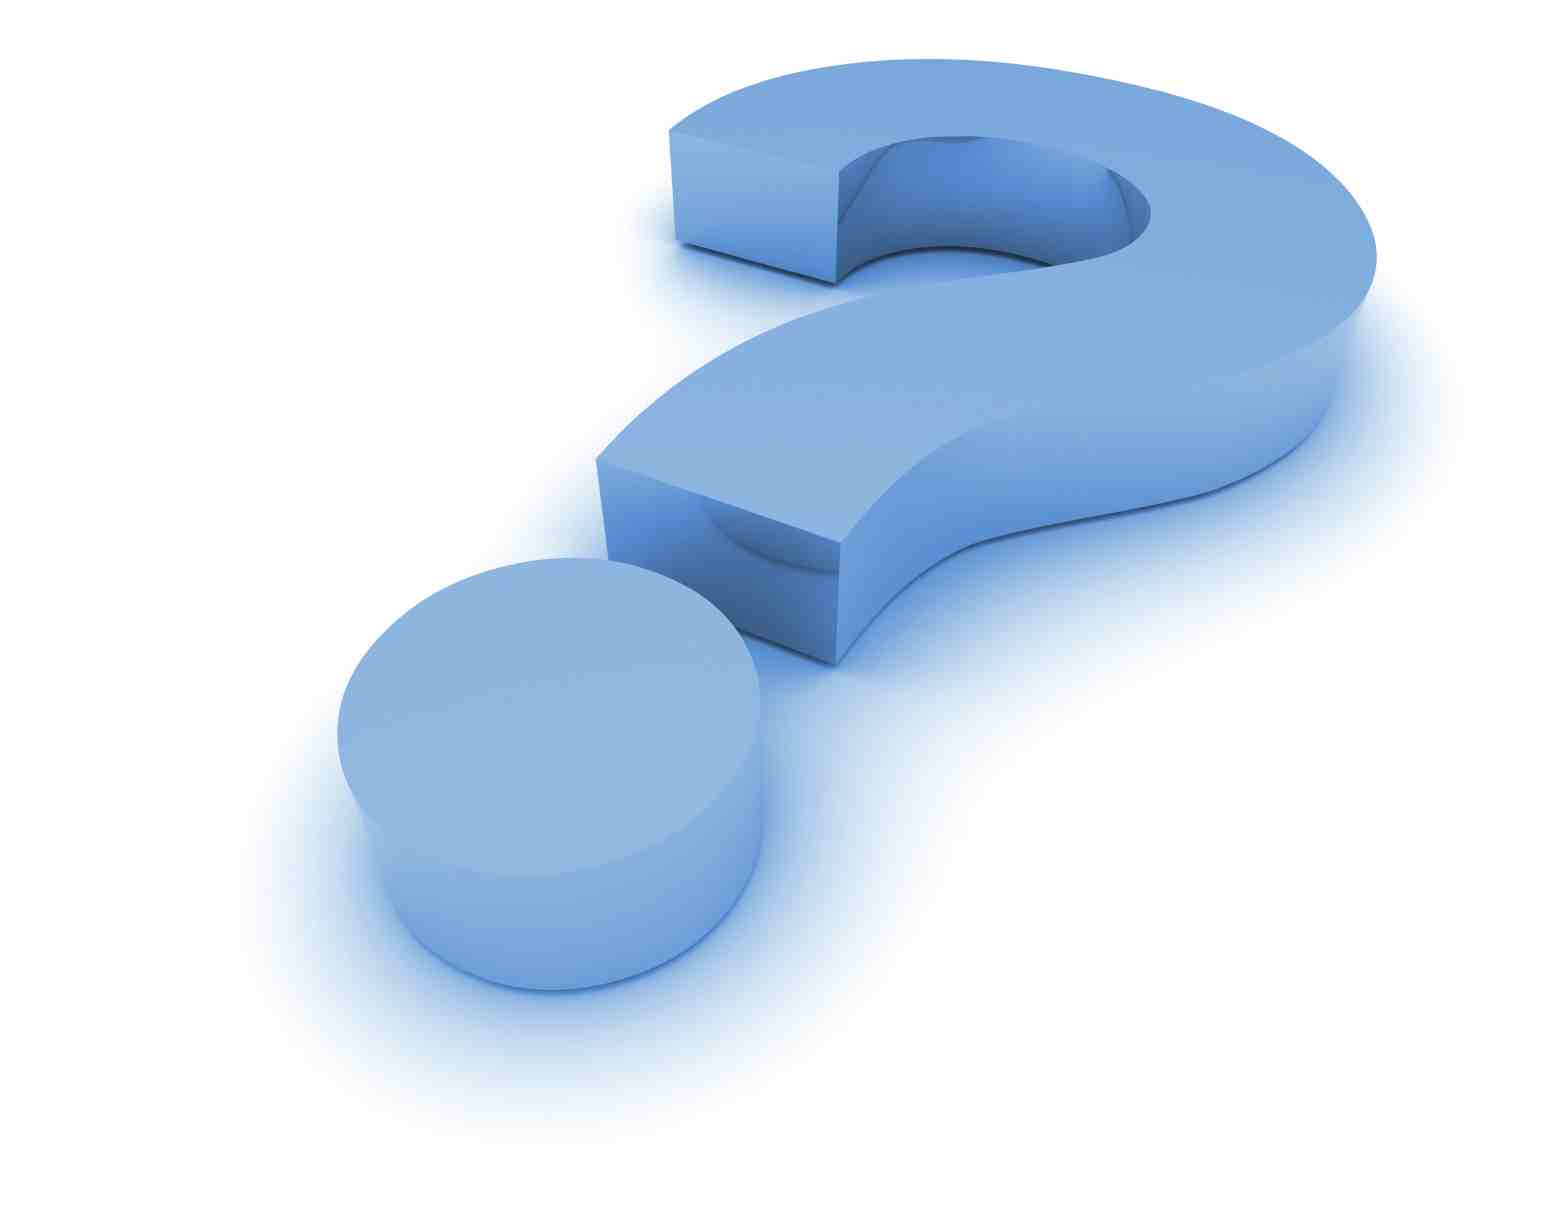
\includegraphics[width=0.8\textwidth]{imagenes/questions}
	}


\end{frame}

\end{document}